
% Default to the notebook output style

    


% Inherit from the specified cell style.




    
\documentclass[11pt]{article}

    
    
    \usepackage[T1]{fontenc}
    % Nicer default font (+ math font) than Computer Modern for most use cases
    \usepackage{mathpazo}

    % Basic figure setup, for now with no caption control since it's done
    % automatically by Pandoc (which extracts ![](path) syntax from Markdown).
    \usepackage{graphicx}
    \usepackage{float}
    % We will generate all images so they have a width \maxwidth. This means
    % that they will get their normal width if they fit onto the page, but
    % are scaled down if they would overflow the margins.
    \makeatletter
    \def\maxwidth{\ifdim\Gin@nat@width>\linewidth\linewidth
    \else\Gin@nat@width\fi}
    \makeatother
    \let\Oldincludegraphics\includegraphics
    % Set max figure width to be 80% of text width, for now hardcoded.
    \renewcommand{\includegraphics}[1]{\Oldincludegraphics[width=.8\maxwidth]{#1}}
    % Ensure that by default, figures have no caption (until we provide a
    % proper Figure object with a Caption API and a way to capture that
    % in the conversion process - todo).
    \usepackage{caption}
    \DeclareCaptionLabelFormat{nolabel}{}
    \captionsetup{labelformat=nolabel}

    \usepackage{adjustbox} % Used to constrain images to a maximum size 
    \usepackage{xcolor} % Allow colors to be defined
    \usepackage{enumerate} % Needed for markdown enumerations to work
    \usepackage{geometry} % Used to adjust the document margins
    \usepackage{amsmath} % Equations
    \usepackage{amssymb} % Equations
    \usepackage{textcomp} % defines textquotesingle
    % Hack from http://tex.stackexchange.com/a/47451/13684:
    \AtBeginDocument{%
        \def\PYZsq{\textquotesingle}% Upright quotes in Pygmentized code
    }
    \usepackage{upquote} % Upright quotes for verbatim code
    \usepackage{eurosym} % defines \euro
    \usepackage[mathletters]{ucs} % Extended unicode (utf-8) support
    \usepackage[utf8x]{inputenc} % Allow utf-8 characters in the tex document
    \usepackage{fancyvrb} % verbatim replacement that allows latex
    \usepackage{grffile} % extends the file name processing of package graphics 
                         % to support a larger range 
    % The hyperref package gives us a pdf with properly built
    % internal navigation ('pdf bookmarks' for the table of contents,
    % internal cross-reference links, web links for URLs, etc.)
    \usepackage{hyperref}
    \usepackage{longtable} % longtable support required by pandoc >1.10
    \usepackage{booktabs}  % table support for pandoc > 1.12.2
    \usepackage[inline]{enumitem} % IRkernel/repr support (it uses the enumerate* environment)
    \usepackage[normalem]{ulem} % ulem is needed to support strikethroughs (\sout)
                                % normalem makes italics be italics, not underlines
    \usepackage{mathrsfs}
    

    
    
    % Colors for the hyperref package
    \definecolor{urlcolor}{rgb}{0,.145,.698}
    \definecolor{linkcolor}{rgb}{.71,0.21,0.01}
    \definecolor{citecolor}{rgb}{.12,.54,.11}

    % ANSI colors
    \definecolor{ansi-black}{HTML}{3E424D}
    \definecolor{ansi-black-intense}{HTML}{282C36}
    \definecolor{ansi-red}{HTML}{E75C58}
    \definecolor{ansi-red-intense}{HTML}{B22B31}
    \definecolor{ansi-green}{HTML}{00A250}
    \definecolor{ansi-green-intense}{HTML}{007427}
    \definecolor{ansi-yellow}{HTML}{DDB62B}
    \definecolor{ansi-yellow-intense}{HTML}{B27D12}
    \definecolor{ansi-blue}{HTML}{208FFB}
    \definecolor{ansi-blue-intense}{HTML}{0065CA}
    \definecolor{ansi-magenta}{HTML}{D160C4}
    \definecolor{ansi-magenta-intense}{HTML}{A03196}
    \definecolor{ansi-cyan}{HTML}{60C6C8}
    \definecolor{ansi-cyan-intense}{HTML}{258F8F}
    \definecolor{ansi-white}{HTML}{C5C1B4}
    \definecolor{ansi-white-intense}{HTML}{A1A6B2}
    \definecolor{ansi-default-inverse-fg}{HTML}{FFFFFF}
    \definecolor{ansi-default-inverse-bg}{HTML}{000000}

    % commands and environments needed by pandoc snippets
    % extracted from the output of `pandoc -s`
    \providecommand{\tightlist}{%
      \setlength{\itemsep}{0pt}\setlength{\parskip}{0pt}}
    \DefineVerbatimEnvironment{Highlighting}{Verbatim}{commandchars=\\\{\}}
    % Add ',fontsize=\small' for more characters per line
    \newenvironment{Shaded}{}{}
    \newcommand{\KeywordTok}[1]{\textcolor[rgb]{0.00,0.44,0.13}{\textbf{{#1}}}}
    \newcommand{\DataTypeTok}[1]{\textcolor[rgb]{0.56,0.13,0.00}{{#1}}}
    \newcommand{\DecValTok}[1]{\textcolor[rgb]{0.25,0.63,0.44}{{#1}}}
    \newcommand{\BaseNTok}[1]{\textcolor[rgb]{0.25,0.63,0.44}{{#1}}}
    \newcommand{\FloatTok}[1]{\textcolor[rgb]{0.25,0.63,0.44}{{#1}}}
    \newcommand{\CharTok}[1]{\textcolor[rgb]{0.25,0.44,0.63}{{#1}}}
    \newcommand{\StringTok}[1]{\textcolor[rgb]{0.25,0.44,0.63}{{#1}}}
    \newcommand{\CommentTok}[1]{\textcolor[rgb]{0.38,0.63,0.69}{\textit{{#1}}}}
    \newcommand{\OtherTok}[1]{\textcolor[rgb]{0.00,0.44,0.13}{{#1}}}
    \newcommand{\AlertTok}[1]{\textcolor[rgb]{1.00,0.00,0.00}{\textbf{{#1}}}}
    \newcommand{\FunctionTok}[1]{\textcolor[rgb]{0.02,0.16,0.49}{{#1}}}
    \newcommand{\RegionMarkerTok}[1]{{#1}}
    \newcommand{\ErrorTok}[1]{\textcolor[rgb]{1.00,0.00,0.00}{\textbf{{#1}}}}
    \newcommand{\NormalTok}[1]{{#1}}
    
    % Additional commands for more recent versions of Pandoc
    \newcommand{\ConstantTok}[1]{\textcolor[rgb]{0.53,0.00,0.00}{{#1}}}
    \newcommand{\SpecialCharTok}[1]{\textcolor[rgb]{0.25,0.44,0.63}{{#1}}}
    \newcommand{\VerbatimStringTok}[1]{\textcolor[rgb]{0.25,0.44,0.63}{{#1}}}
    \newcommand{\SpecialStringTok}[1]{\textcolor[rgb]{0.73,0.40,0.53}{{#1}}}
    \newcommand{\ImportTok}[1]{{#1}}
    \newcommand{\DocumentationTok}[1]{\textcolor[rgb]{0.73,0.13,0.13}{\textit{{#1}}}}
    \newcommand{\AnnotationTok}[1]{\textcolor[rgb]{0.38,0.63,0.69}{\textbf{\textit{{#1}}}}}
    \newcommand{\CommentVarTok}[1]{\textcolor[rgb]{0.38,0.63,0.69}{\textbf{\textit{{#1}}}}}
    \newcommand{\VariableTok}[1]{\textcolor[rgb]{0.10,0.09,0.49}{{#1}}}
    \newcommand{\ControlFlowTok}[1]{\textcolor[rgb]{0.00,0.44,0.13}{\textbf{{#1}}}}
    \newcommand{\OperatorTok}[1]{\textcolor[rgb]{0.40,0.40,0.40}{{#1}}}
    \newcommand{\BuiltInTok}[1]{{#1}}
    \newcommand{\ExtensionTok}[1]{{#1}}
    \newcommand{\PreprocessorTok}[1]{\textcolor[rgb]{0.74,0.48,0.00}{{#1}}}
    \newcommand{\AttributeTok}[1]{\textcolor[rgb]{0.49,0.56,0.16}{{#1}}}
    \newcommand{\InformationTok}[1]{\textcolor[rgb]{0.38,0.63,0.69}{\textbf{\textit{{#1}}}}}
    \newcommand{\WarningTok}[1]{\textcolor[rgb]{0.38,0.63,0.69}{\textbf{\textit{{#1}}}}}
    
    
    % Define a nice break command that doesn't care if a line doesn't already
    % exist.
    \def\br{\hspace*{\fill} \\* }
    % Math Jax compatibility definitions
    \def\gt{>}
    \def\lt{<}
    \let\Oldtex\TeX
    \let\Oldlatex\LaTeX
    \renewcommand{\TeX}{\textrm{\Oldtex}}
    \renewcommand{\LaTeX}{\textrm{\Oldlatex}}
    % Document parameters
    % Document title
    \title{Assignment 11}
    
    
    
    \author{Jiarong Ye}
    

    % Pygments definitions
    
\makeatletter
\def\PY@reset{\let\PY@it=\relax \let\PY@bf=\relax%
    \let\PY@ul=\relax \let\PY@tc=\relax%
    \let\PY@bc=\relax \let\PY@ff=\relax}
\def\PY@tok#1{\csname PY@tok@#1\endcsname}
\def\PY@toks#1+{\ifx\relax#1\empty\else%
    \PY@tok{#1}\expandafter\PY@toks\fi}
\def\PY@do#1{\PY@bc{\PY@tc{\PY@ul{%
    \PY@it{\PY@bf{\PY@ff{#1}}}}}}}
\def\PY#1#2{\PY@reset\PY@toks#1+\relax+\PY@do{#2}}

\expandafter\def\csname PY@tok@w\endcsname{\def\PY@tc##1{\textcolor[rgb]{0.73,0.73,0.73}{##1}}}
\expandafter\def\csname PY@tok@c\endcsname{\let\PY@it=\textit\def\PY@tc##1{\textcolor[rgb]{0.25,0.50,0.50}{##1}}}
\expandafter\def\csname PY@tok@cp\endcsname{\def\PY@tc##1{\textcolor[rgb]{0.74,0.48,0.00}{##1}}}
\expandafter\def\csname PY@tok@k\endcsname{\let\PY@bf=\textbf\def\PY@tc##1{\textcolor[rgb]{0.00,0.50,0.00}{##1}}}
\expandafter\def\csname PY@tok@kp\endcsname{\def\PY@tc##1{\textcolor[rgb]{0.00,0.50,0.00}{##1}}}
\expandafter\def\csname PY@tok@kt\endcsname{\def\PY@tc##1{\textcolor[rgb]{0.69,0.00,0.25}{##1}}}
\expandafter\def\csname PY@tok@o\endcsname{\def\PY@tc##1{\textcolor[rgb]{0.40,0.40,0.40}{##1}}}
\expandafter\def\csname PY@tok@ow\endcsname{\let\PY@bf=\textbf\def\PY@tc##1{\textcolor[rgb]{0.67,0.13,1.00}{##1}}}
\expandafter\def\csname PY@tok@nb\endcsname{\def\PY@tc##1{\textcolor[rgb]{0.00,0.50,0.00}{##1}}}
\expandafter\def\csname PY@tok@nf\endcsname{\def\PY@tc##1{\textcolor[rgb]{0.00,0.00,1.00}{##1}}}
\expandafter\def\csname PY@tok@nc\endcsname{\let\PY@bf=\textbf\def\PY@tc##1{\textcolor[rgb]{0.00,0.00,1.00}{##1}}}
\expandafter\def\csname PY@tok@nn\endcsname{\let\PY@bf=\textbf\def\PY@tc##1{\textcolor[rgb]{0.00,0.00,1.00}{##1}}}
\expandafter\def\csname PY@tok@ne\endcsname{\let\PY@bf=\textbf\def\PY@tc##1{\textcolor[rgb]{0.82,0.25,0.23}{##1}}}
\expandafter\def\csname PY@tok@nv\endcsname{\def\PY@tc##1{\textcolor[rgb]{0.10,0.09,0.49}{##1}}}
\expandafter\def\csname PY@tok@no\endcsname{\def\PY@tc##1{\textcolor[rgb]{0.53,0.00,0.00}{##1}}}
\expandafter\def\csname PY@tok@nl\endcsname{\def\PY@tc##1{\textcolor[rgb]{0.63,0.63,0.00}{##1}}}
\expandafter\def\csname PY@tok@ni\endcsname{\let\PY@bf=\textbf\def\PY@tc##1{\textcolor[rgb]{0.60,0.60,0.60}{##1}}}
\expandafter\def\csname PY@tok@na\endcsname{\def\PY@tc##1{\textcolor[rgb]{0.49,0.56,0.16}{##1}}}
\expandafter\def\csname PY@tok@nt\endcsname{\let\PY@bf=\textbf\def\PY@tc##1{\textcolor[rgb]{0.00,0.50,0.00}{##1}}}
\expandafter\def\csname PY@tok@nd\endcsname{\def\PY@tc##1{\textcolor[rgb]{0.67,0.13,1.00}{##1}}}
\expandafter\def\csname PY@tok@s\endcsname{\def\PY@tc##1{\textcolor[rgb]{0.73,0.13,0.13}{##1}}}
\expandafter\def\csname PY@tok@sd\endcsname{\let\PY@it=\textit\def\PY@tc##1{\textcolor[rgb]{0.73,0.13,0.13}{##1}}}
\expandafter\def\csname PY@tok@si\endcsname{\let\PY@bf=\textbf\def\PY@tc##1{\textcolor[rgb]{0.73,0.40,0.53}{##1}}}
\expandafter\def\csname PY@tok@se\endcsname{\let\PY@bf=\textbf\def\PY@tc##1{\textcolor[rgb]{0.73,0.40,0.13}{##1}}}
\expandafter\def\csname PY@tok@sr\endcsname{\def\PY@tc##1{\textcolor[rgb]{0.73,0.40,0.53}{##1}}}
\expandafter\def\csname PY@tok@ss\endcsname{\def\PY@tc##1{\textcolor[rgb]{0.10,0.09,0.49}{##1}}}
\expandafter\def\csname PY@tok@sx\endcsname{\def\PY@tc##1{\textcolor[rgb]{0.00,0.50,0.00}{##1}}}
\expandafter\def\csname PY@tok@m\endcsname{\def\PY@tc##1{\textcolor[rgb]{0.40,0.40,0.40}{##1}}}
\expandafter\def\csname PY@tok@gh\endcsname{\let\PY@bf=\textbf\def\PY@tc##1{\textcolor[rgb]{0.00,0.00,0.50}{##1}}}
\expandafter\def\csname PY@tok@gu\endcsname{\let\PY@bf=\textbf\def\PY@tc##1{\textcolor[rgb]{0.50,0.00,0.50}{##1}}}
\expandafter\def\csname PY@tok@gd\endcsname{\def\PY@tc##1{\textcolor[rgb]{0.63,0.00,0.00}{##1}}}
\expandafter\def\csname PY@tok@gi\endcsname{\def\PY@tc##1{\textcolor[rgb]{0.00,0.63,0.00}{##1}}}
\expandafter\def\csname PY@tok@gr\endcsname{\def\PY@tc##1{\textcolor[rgb]{1.00,0.00,0.00}{##1}}}
\expandafter\def\csname PY@tok@ge\endcsname{\let\PY@it=\textit}
\expandafter\def\csname PY@tok@gs\endcsname{\let\PY@bf=\textbf}
\expandafter\def\csname PY@tok@gp\endcsname{\let\PY@bf=\textbf\def\PY@tc##1{\textcolor[rgb]{0.00,0.00,0.50}{##1}}}
\expandafter\def\csname PY@tok@go\endcsname{\def\PY@tc##1{\textcolor[rgb]{0.53,0.53,0.53}{##1}}}
\expandafter\def\csname PY@tok@gt\endcsname{\def\PY@tc##1{\textcolor[rgb]{0.00,0.27,0.87}{##1}}}
\expandafter\def\csname PY@tok@err\endcsname{\def\PY@bc##1{\setlength{\fboxsep}{0pt}\fcolorbox[rgb]{1.00,0.00,0.00}{1,1,1}{\strut ##1}}}
\expandafter\def\csname PY@tok@kc\endcsname{\let\PY@bf=\textbf\def\PY@tc##1{\textcolor[rgb]{0.00,0.50,0.00}{##1}}}
\expandafter\def\csname PY@tok@kd\endcsname{\let\PY@bf=\textbf\def\PY@tc##1{\textcolor[rgb]{0.00,0.50,0.00}{##1}}}
\expandafter\def\csname PY@tok@kn\endcsname{\let\PY@bf=\textbf\def\PY@tc##1{\textcolor[rgb]{0.00,0.50,0.00}{##1}}}
\expandafter\def\csname PY@tok@kr\endcsname{\let\PY@bf=\textbf\def\PY@tc##1{\textcolor[rgb]{0.00,0.50,0.00}{##1}}}
\expandafter\def\csname PY@tok@bp\endcsname{\def\PY@tc##1{\textcolor[rgb]{0.00,0.50,0.00}{##1}}}
\expandafter\def\csname PY@tok@fm\endcsname{\def\PY@tc##1{\textcolor[rgb]{0.00,0.00,1.00}{##1}}}
\expandafter\def\csname PY@tok@vc\endcsname{\def\PY@tc##1{\textcolor[rgb]{0.10,0.09,0.49}{##1}}}
\expandafter\def\csname PY@tok@vg\endcsname{\def\PY@tc##1{\textcolor[rgb]{0.10,0.09,0.49}{##1}}}
\expandafter\def\csname PY@tok@vi\endcsname{\def\PY@tc##1{\textcolor[rgb]{0.10,0.09,0.49}{##1}}}
\expandafter\def\csname PY@tok@vm\endcsname{\def\PY@tc##1{\textcolor[rgb]{0.10,0.09,0.49}{##1}}}
\expandafter\def\csname PY@tok@sa\endcsname{\def\PY@tc##1{\textcolor[rgb]{0.73,0.13,0.13}{##1}}}
\expandafter\def\csname PY@tok@sb\endcsname{\def\PY@tc##1{\textcolor[rgb]{0.73,0.13,0.13}{##1}}}
\expandafter\def\csname PY@tok@sc\endcsname{\def\PY@tc##1{\textcolor[rgb]{0.73,0.13,0.13}{##1}}}
\expandafter\def\csname PY@tok@dl\endcsname{\def\PY@tc##1{\textcolor[rgb]{0.73,0.13,0.13}{##1}}}
\expandafter\def\csname PY@tok@s2\endcsname{\def\PY@tc##1{\textcolor[rgb]{0.73,0.13,0.13}{##1}}}
\expandafter\def\csname PY@tok@sh\endcsname{\def\PY@tc##1{\textcolor[rgb]{0.73,0.13,0.13}{##1}}}
\expandafter\def\csname PY@tok@s1\endcsname{\def\PY@tc##1{\textcolor[rgb]{0.73,0.13,0.13}{##1}}}
\expandafter\def\csname PY@tok@mb\endcsname{\def\PY@tc##1{\textcolor[rgb]{0.40,0.40,0.40}{##1}}}
\expandafter\def\csname PY@tok@mf\endcsname{\def\PY@tc##1{\textcolor[rgb]{0.40,0.40,0.40}{##1}}}
\expandafter\def\csname PY@tok@mh\endcsname{\def\PY@tc##1{\textcolor[rgb]{0.40,0.40,0.40}{##1}}}
\expandafter\def\csname PY@tok@mi\endcsname{\def\PY@tc##1{\textcolor[rgb]{0.40,0.40,0.40}{##1}}}
\expandafter\def\csname PY@tok@il\endcsname{\def\PY@tc##1{\textcolor[rgb]{0.40,0.40,0.40}{##1}}}
\expandafter\def\csname PY@tok@mo\endcsname{\def\PY@tc##1{\textcolor[rgb]{0.40,0.40,0.40}{##1}}}
\expandafter\def\csname PY@tok@ch\endcsname{\let\PY@it=\textit\def\PY@tc##1{\textcolor[rgb]{0.25,0.50,0.50}{##1}}}
\expandafter\def\csname PY@tok@cm\endcsname{\let\PY@it=\textit\def\PY@tc##1{\textcolor[rgb]{0.25,0.50,0.50}{##1}}}
\expandafter\def\csname PY@tok@cpf\endcsname{\let\PY@it=\textit\def\PY@tc##1{\textcolor[rgb]{0.25,0.50,0.50}{##1}}}
\expandafter\def\csname PY@tok@c1\endcsname{\let\PY@it=\textit\def\PY@tc##1{\textcolor[rgb]{0.25,0.50,0.50}{##1}}}
\expandafter\def\csname PY@tok@cs\endcsname{\let\PY@it=\textit\def\PY@tc##1{\textcolor[rgb]{0.25,0.50,0.50}{##1}}}

\def\PYZbs{\char`\\}
\def\PYZus{\char`\_}
\def\PYZob{\char`\{}
\def\PYZcb{\char`\}}
\def\PYZca{\char`\^}
\def\PYZam{\char`\&}
\def\PYZlt{\char`\<}
\def\PYZgt{\char`\>}
\def\PYZsh{\char`\#}
\def\PYZpc{\char`\%}
\def\PYZdl{\char`\$}
\def\PYZhy{\char`\-}
\def\PYZsq{\char`\'}
\def\PYZdq{\char`\"}
\def\PYZti{\char`\~}
% for compatibility with earlier versions
\def\PYZat{@}
\def\PYZlb{[}
\def\PYZrb{]}
\makeatother


    % Exact colors from NB
    \definecolor{incolor}{rgb}{0.0, 0.0, 0.5}
    \definecolor{outcolor}{rgb}{0.545, 0.0, 0.0}



    
    % Prevent overflowing lines due to hard-to-break entities
    \sloppy 
    % Setup hyperref package
    \hypersetup{
      breaklinks=true,  % so long urls are correctly broken across lines
      colorlinks=true,
      urlcolor=urlcolor,
      linkcolor=linkcolor,
      citecolor=citecolor,
      }
    % Slightly bigger margins than the latex defaults
    
    \geometry{verbose,tmargin=1in,bmargin=1in,lmargin=1in,rmargin=1in,left=1cm, right=1cm}
    
    

    \begin{document}
    
    
    \maketitle
    
    

    
    \subsection*{Q1}\label{q1}

A ER diagram showing your data table design in 3NF.

    \begin{figure}[H]
\centering
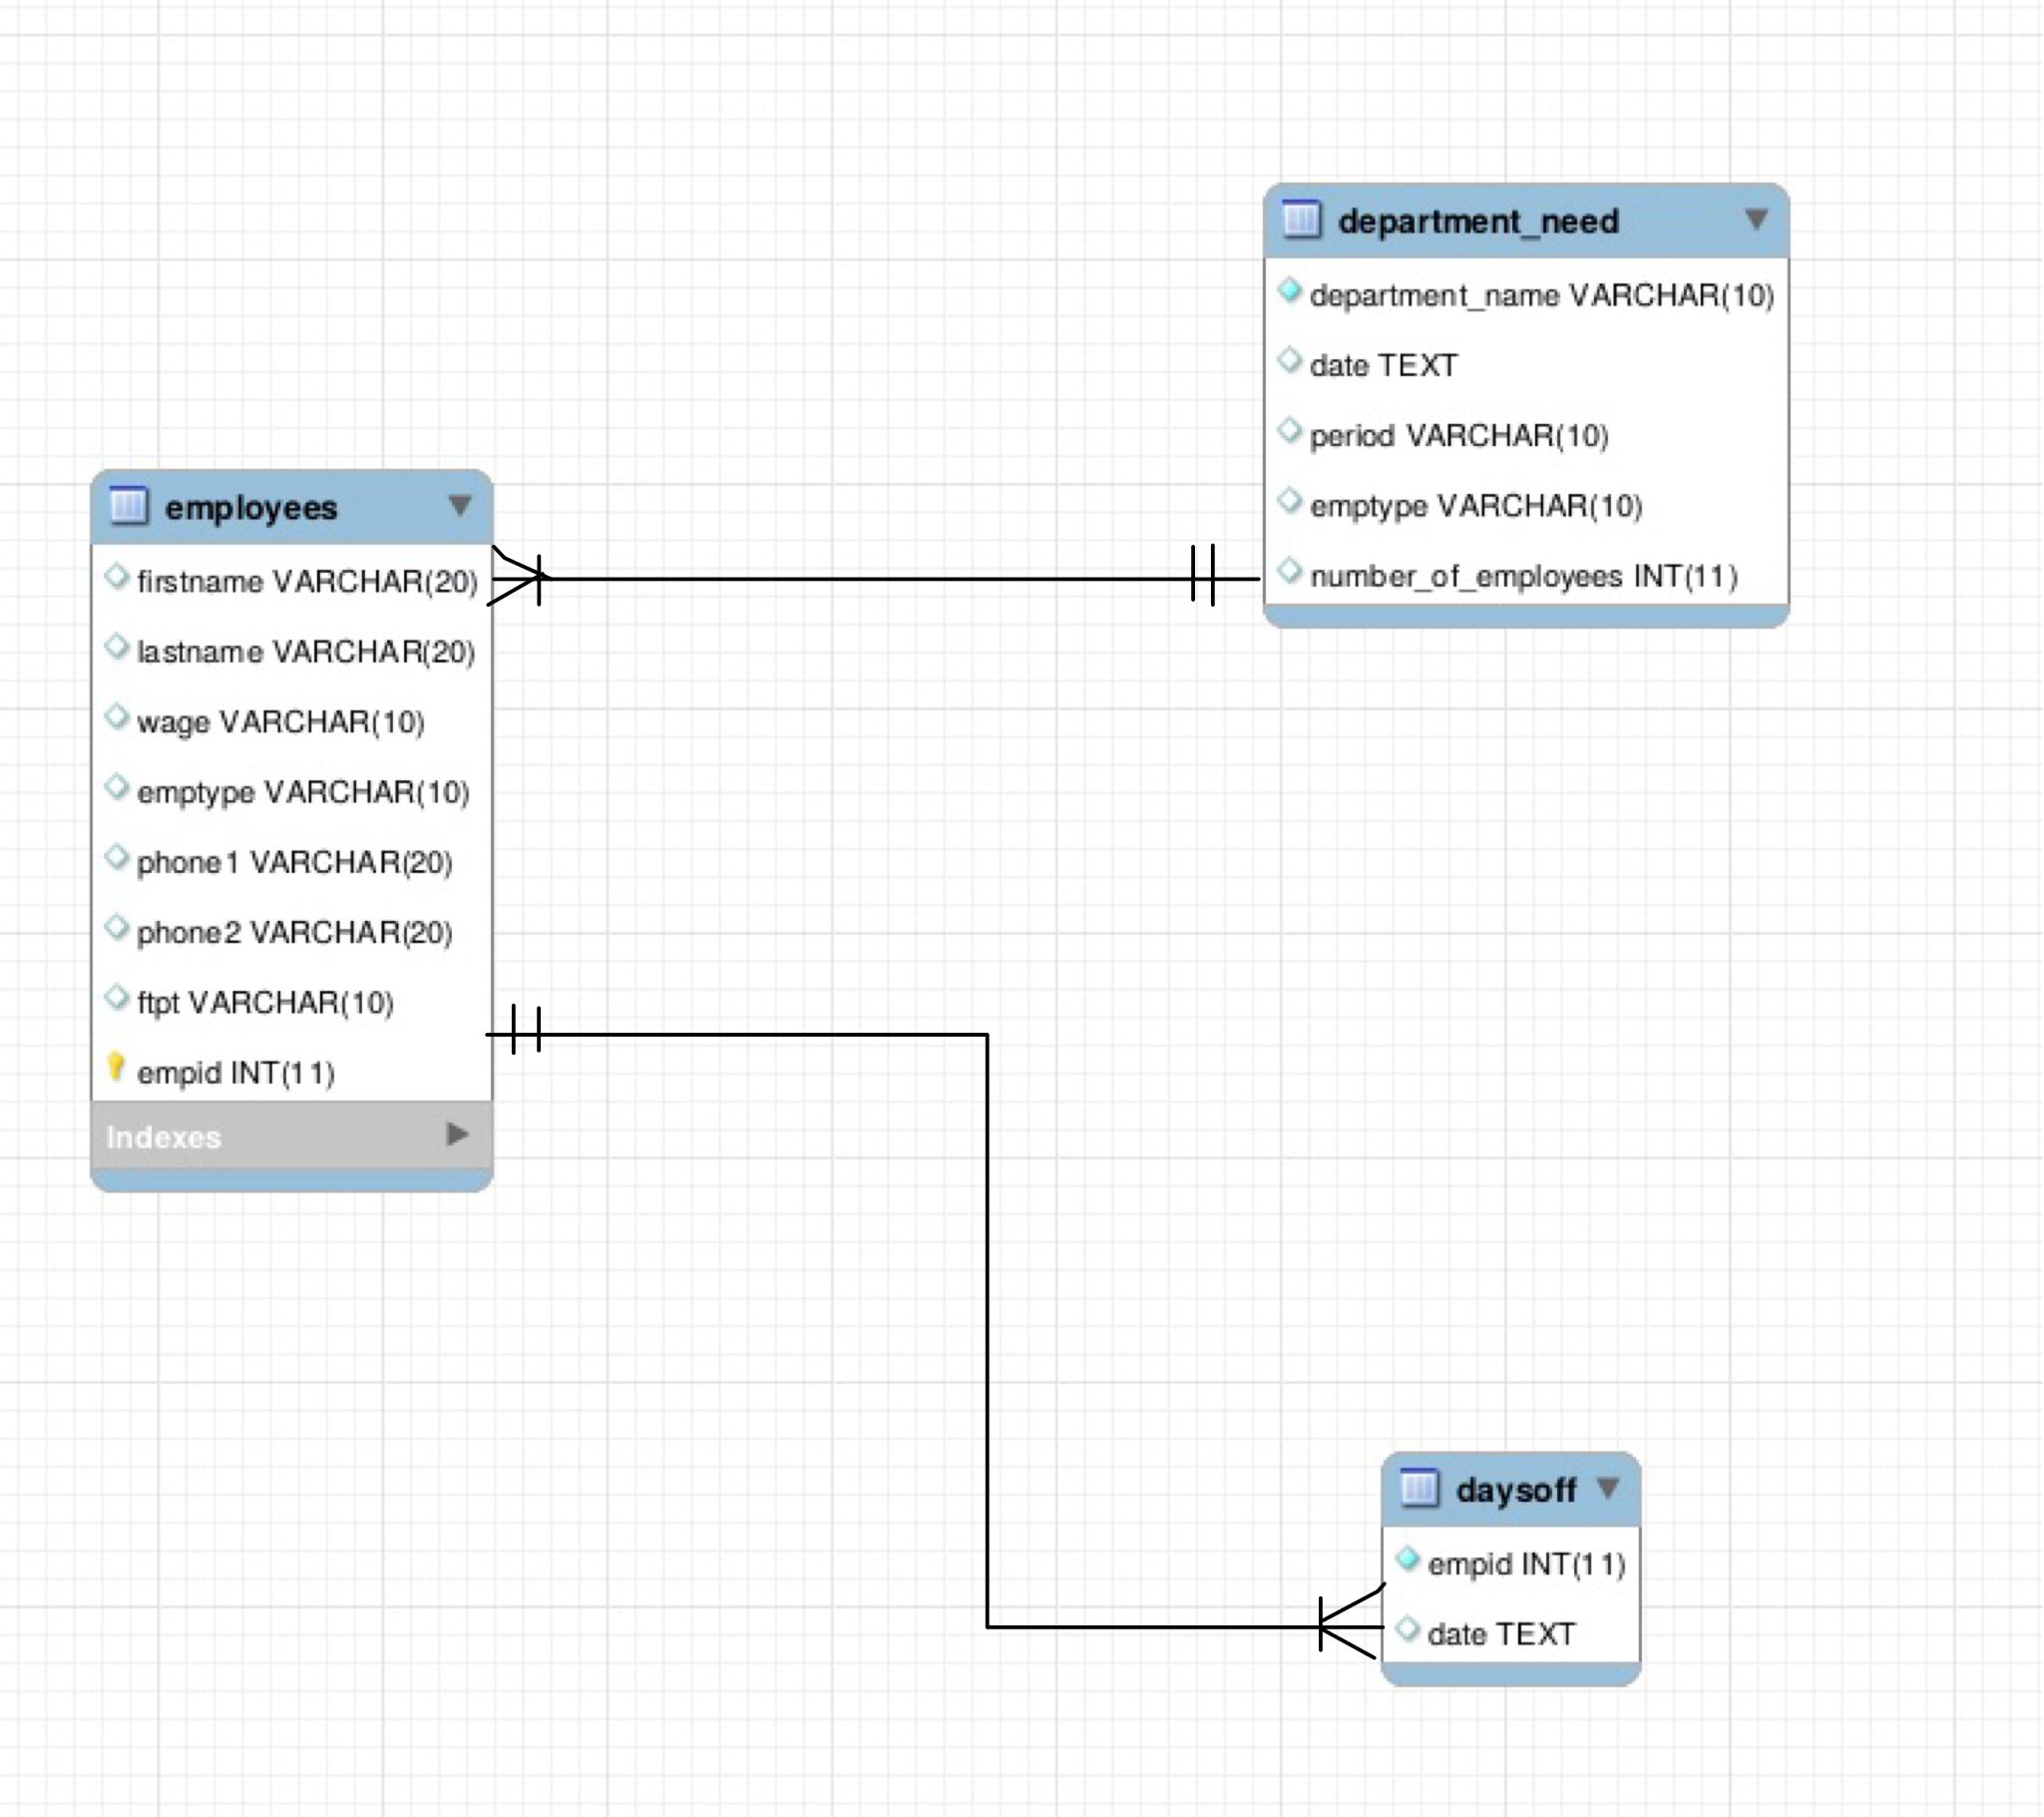
\includegraphics{1.png}
\caption{}
\end{figure}

    \subsection*{Q2}\label{q2}

Load this data into your 3NF tables structure.

    \begin{Verbatim}[commandchars=\\\{\}]
{\color{incolor}In [{\color{incolor}4}]:} \PY{n}{CREATE} \PY{n}{TABLE} \PY{n}{department\PYZus{}need}
        \PY{p}{(}
          \PY{n}{department\PYZus{}name}  \PY{n}{VARCHAR}\PY{p}{(}\PY{l+m+mi}{10}\PY{p}{)} \PY{n}{NOT} \PY{n}{NULL}\PY{p}{,}
          \PY{n}{date}             \PY{n}{TEXT}        \PY{n}{NULL}\PY{p}{,}
          \PY{n}{period}           \PY{n}{VARCHAR}\PY{p}{(}\PY{l+m+mi}{10}\PY{p}{)} \PY{n}{NULL}\PY{p}{,}
          \PY{n}{emptype}          \PY{n}{VARCHAR}\PY{p}{(}\PY{l+m+mi}{10}\PY{p}{)} \PY{n}{NULL}\PY{p}{,}
          \PY{n}{number\PYZus{}of\PYZus{}employees}  \PY{n}{INT}     \PY{n}{NULL}
        \PY{p}{)}\PY{p}{;}
        
        \PY{n}{CREATE} \PY{n}{TABLE} \PY{n}{employees}
        \PY{p}{(}
          \PY{n}{firstname} \PY{n}{VARCHAR}\PY{p}{(}\PY{l+m+mi}{20}\PY{p}{)} \PY{n}{NULL}\PY{p}{,}
          \PY{n}{lastname}  \PY{n}{VARCHAR}\PY{p}{(}\PY{l+m+mi}{20}\PY{p}{)} \PY{n}{NULL}\PY{p}{,}
          \PY{n}{wage}      \PY{n}{VARCHAR}\PY{p}{(}\PY{l+m+mi}{10}\PY{p}{)} \PY{n}{NULL}\PY{p}{,}
          \PY{n}{emptype}   \PY{n}{VARCHAR}\PY{p}{(}\PY{l+m+mi}{10}\PY{p}{)} \PY{n}{NULL}\PY{p}{,}
          \PY{n}{phone1}    \PY{n}{VARCHAR}\PY{p}{(}\PY{l+m+mi}{20}\PY{p}{)} \PY{n}{NULL}\PY{p}{,}
          \PY{n}{phone2}    \PY{n}{VARCHAR}\PY{p}{(}\PY{l+m+mi}{20}\PY{p}{)} \PY{n}{NULL}\PY{p}{,}
          \PY{n}{ftpt}      \PY{n}{VARCHAR}\PY{p}{(}\PY{l+m+mi}{10}\PY{p}{)}  \PY{n}{NULL}
        \PY{p}{)}\PY{p}{;}
        
        
        \PY{n}{CREATE} \PY{n}{TABLE} \PY{n}{daysoff}
        \PY{p}{(}
          \PY{n}{firstname} \PY{n}{VARCHAR}\PY{p}{(}\PY{l+m+mi}{20}\PY{p}{)} \PY{n}{NOT} \PY{n}{NULL}\PY{p}{,}
          \PY{n}{lastname}  \PY{n}{VARCHAR}\PY{p}{(}\PY{l+m+mi}{20}\PY{p}{)} \PY{n}{NOT} \PY{n}{NULL}\PY{p}{,}
          \PY{n}{date}  \PY{n}{TEXT} \PY{n}{NULL}
        \PY{p}{)}\PY{p}{;}
        
        
        
        \PY{n}{LOAD} \PY{n}{DATA} \PY{n}{INFILE} \PY{l+s+s1}{\PYZsq{}}\PY{l+s+s1}{project\PYZus{}asgn\PYZus{}11\PYZus{}data/needs.csv}\PY{l+s+s1}{\PYZsq{}} \PY{n}{INTO} \PY{n}{TABLE} \PY{n}{department\PYZus{}need}
        \PY{n}{FIELDS} \PY{n}{TERMINATED} \PY{n}{BY} \PY{l+s+s1}{\PYZsq{}}\PY{l+s+s1}{,}\PY{l+s+s1}{\PYZsq{}} \PY{n}{LINES} \PY{n}{TERMINATED} \PY{n}{BY} \PY{l+s+s1}{\PYZsq{}}\PY{l+s+se}{\PYZbs{}r}\PY{l+s+se}{\PYZbs{}n}\PY{l+s+s1}{\PYZsq{}}\PY{p}{;}
        
        
        \PY{n}{LOAD} \PY{n}{DATA} \PY{n}{INFILE} \PY{l+s+s1}{\PYZsq{}}\PY{l+s+s1}{project\PYZus{}asgn\PYZus{}11\PYZus{}data/employee2.csv}\PY{l+s+s1}{\PYZsq{}} \PY{n}{INTO} \PY{n}{TABLE} \PY{n}{employees}
        \PY{n}{FIELDS} \PY{n}{TERMINATED} \PY{n}{BY} \PY{l+s+s1}{\PYZsq{}}\PY{l+s+s1}{,}\PY{l+s+s1}{\PYZsq{}} \PY{n}{LINES} \PY{n}{TERMINATED} \PY{n}{BY} \PY{l+s+s1}{\PYZsq{}}\PY{l+s+se}{\PYZbs{}r}\PY{l+s+se}{\PYZbs{}n}\PY{l+s+s1}{\PYZsq{}}\PY{p}{;}
        
        
        \PY{n}{LOAD} \PY{n}{DATA} \PY{n}{INFILE} \PY{l+s+s1}{\PYZsq{}}\PY{l+s+s1}{project\PYZus{}asgn\PYZus{}11\PYZus{}data/daysoffrequests.csv}\PY{l+s+s1}{\PYZsq{}} \PY{n}{INTO} \PY{n}{TABLE} \PY{n}{daysoff}
        \PY{n}{FIELDS} \PY{n}{TERMINATED} \PY{n}{BY} \PY{l+s+s1}{\PYZsq{}}\PY{l+s+s1}{,}\PY{l+s+s1}{\PYZsq{}} \PY{n}{LINES} \PY{n}{TERMINATED} \PY{n}{BY} \PY{l+s+s1}{\PYZsq{}}\PY{l+s+se}{\PYZbs{}r}\PY{l+s+se}{\PYZbs{}n}\PY{l+s+s1}{\PYZsq{}}\PY{p}{;}
        
        
        \PY{n}{UPDATE} \PY{n}{daysoff} \PY{n}{SET} \PY{n}{firstname} \PY{o}{=} \PY{n}{REPLACE}\PY{p}{(}\PY{n}{firstname}\PY{p}{,} \PY{l+s+s1}{\PYZsq{}}\PY{l+s+s1}{ }\PY{l+s+s1}{\PYZsq{}}\PY{p}{,} \PY{l+s+s1}{\PYZsq{}}\PY{l+s+s1}{\PYZsq{}}\PY{p}{)}\PY{p}{;}
        \PY{n}{UPDATE} \PY{n}{employees} \PY{n}{SET} \PY{n}{firstname} \PY{o}{=} \PY{n}{REPLACE}\PY{p}{(}\PY{n}{firstname}\PY{p}{,} \PY{l+s+s1}{\PYZsq{}}\PY{l+s+s1}{\PYZdq{}}\PY{l+s+s1}{\PYZsq{}}\PY{p}{,} \PY{l+s+s1}{\PYZsq{}}\PY{l+s+s1}{\PYZsq{}}\PY{p}{)}\PY{p}{;}
        \PY{n}{UPDATE} \PY{n}{employees} \PY{n}{SET} \PY{n}{lastname} \PY{o}{=} \PY{n}{REPLACE}\PY{p}{(}\PY{n}{lastname}\PY{p}{,} \PY{l+s+s1}{\PYZsq{}}\PY{l+s+s1}{\PYZdq{}}\PY{l+s+s1}{\PYZsq{}}\PY{p}{,} \PY{l+s+s1}{\PYZsq{}}\PY{l+s+s1}{\PYZsq{}}\PY{p}{)}\PY{p}{;}
        \PY{n}{UPDATE} \PY{n}{employees} \PY{n}{SET} \PY{n}{wage} \PY{o}{=} \PY{n}{REPLACE}\PY{p}{(}\PY{n}{wage}\PY{p}{,} \PY{l+s+s1}{\PYZsq{}}\PY{l+s+s1}{\PYZdq{}}\PY{l+s+s1}{\PYZsq{}}\PY{p}{,} \PY{l+s+s1}{\PYZsq{}}\PY{l+s+s1}{\PYZsq{}}\PY{p}{)}\PY{p}{;}
        \PY{n}{UPDATE} \PY{n}{employees} \PY{n}{SET} \PY{n}{wage} \PY{o}{=} \PY{n}{REPLACE}\PY{p}{(}\PY{n}{wage}\PY{p}{,} \PY{l+s+s1}{\PYZsq{}}\PY{l+s+s1}{\PYZdl{}}\PY{l+s+s1}{\PYZsq{}}\PY{p}{,} \PY{l+s+s1}{\PYZsq{}}\PY{l+s+s1}{\PYZsq{}}\PY{p}{)}\PY{p}{;}
        \PY{n}{UPDATE} \PY{n}{employees} \PY{n}{SET} \PY{n}{emptype} \PY{o}{=} \PY{n}{REPLACE}\PY{p}{(}\PY{n}{emptype}\PY{p}{,} \PY{l+s+s1}{\PYZsq{}}\PY{l+s+s1}{\PYZdq{}}\PY{l+s+s1}{\PYZsq{}}\PY{p}{,} \PY{l+s+s1}{\PYZsq{}}\PY{l+s+s1}{\PYZsq{}}\PY{p}{)}\PY{p}{;}
        \PY{n}{UPDATE} \PY{n}{employees} \PY{n}{SET} \PY{n}{phone1} \PY{o}{=} \PY{n}{REPLACE}\PY{p}{(}\PY{n}{phone1}\PY{p}{,} \PY{l+s+s1}{\PYZsq{}}\PY{l+s+s1}{\PYZdq{}}\PY{l+s+s1}{\PYZsq{}}\PY{p}{,} \PY{l+s+s1}{\PYZsq{}}\PY{l+s+s1}{\PYZsq{}}\PY{p}{)}\PY{p}{;}
        \PY{n}{UPDATE} \PY{n}{employees} \PY{n}{SET} \PY{n}{phone2} \PY{o}{=} \PY{n}{REPLACE}\PY{p}{(}\PY{n}{phone2}\PY{p}{,} \PY{l+s+s1}{\PYZsq{}}\PY{l+s+s1}{\PYZdq{}}\PY{l+s+s1}{\PYZsq{}}\PY{p}{,} \PY{l+s+s1}{\PYZsq{}}\PY{l+s+s1}{\PYZsq{}}\PY{p}{)}\PY{p}{;}
        \PY{n}{UPDATE} \PY{n}{employees} \PY{n}{SET} \PY{n}{ftpt} \PY{o}{=} \PY{n}{REPLACE}\PY{p}{(}\PY{n}{ftpt}\PY{p}{,} \PY{l+s+s1}{\PYZsq{}}\PY{l+s+s1}{\PYZdq{}}\PY{l+s+s1}{\PYZsq{}}\PY{p}{,} \PY{l+s+s1}{\PYZsq{}}\PY{l+s+s1}{\PYZsq{}}\PY{p}{)}\PY{p}{;}
        
        
        \PY{n}{ALTER} \PY{n}{TABLE} \PY{n}{employees} \PY{n}{ADD} \PY{n}{empid} \PY{n}{INT} \PY{n}{NOT} \PY{n}{NULL} \PY{n}{AUTO\PYZus{}INCREMENT} \PY{n}{PRIMARY} \PY{n}{KEY}\PY{p}{;}
        
        \PY{n}{CREATE} \PY{n}{TABLE} \PY{n}{daysoff\PYZus{}tmp}
        \PY{p}{(}
          \PY{n}{empid} \PY{n}{INT}  \PY{n}{NOT} \PY{n}{NULL}\PY{p}{,}
          \PY{n}{date}  \PY{n}{TEXT} \PY{n}{NULL}
        \PY{p}{)} \PY{n}{SELECT} \PY{n}{e}\PY{o}{.}\PY{n}{empid}\PY{p}{,} \PY{n}{d}\PY{o}{.}\PY{n}{date}
          \PY{n}{FROM} \PY{n}{employees} \PY{k}{as} \PY{n}{e}\PY{p}{,} \PY{n}{daysoff} \PY{k}{as} \PY{n}{d}
          \PY{n}{WHERE} \PY{p}{(}\PY{n}{d}\PY{o}{.}\PY{n}{firstname}\PY{p}{,} \PY{n}{d}\PY{o}{.}\PY{n}{lastname}\PY{p}{)} \PY{o}{=} \PY{p}{(}\PY{n}{e}\PY{o}{.}\PY{n}{firstname}\PY{p}{,} \PY{n}{e}\PY{o}{.}\PY{n}{lastname}\PY{p}{)}\PY{p}{;}
        
        \PY{n}{DROP} \PY{n}{TABLE} \PY{n}{daysoff}\PY{p}{;}
        \PY{n}{RENAME} \PY{n}{TABLE} \PY{n}{daysoff\PYZus{}tmp} \PY{n}{TO} \PY{n}{daysoff}\PY{p}{;}
        
        \PY{n}{SHOW} \PY{n}{TABLES}\PY{p}{;}
        \PY{n}{DESCRIBE} \PY{n}{department\PYZus{}need}\PY{p}{;}
        \PY{n}{DESCRIBE} \PY{n}{employees}\PY{p}{;}
        \PY{n}{DESCRIBE} \PY{n}{daysoff}\PY{p}{;}
\end{Verbatim}

    \begin{figure}[H]
\centering
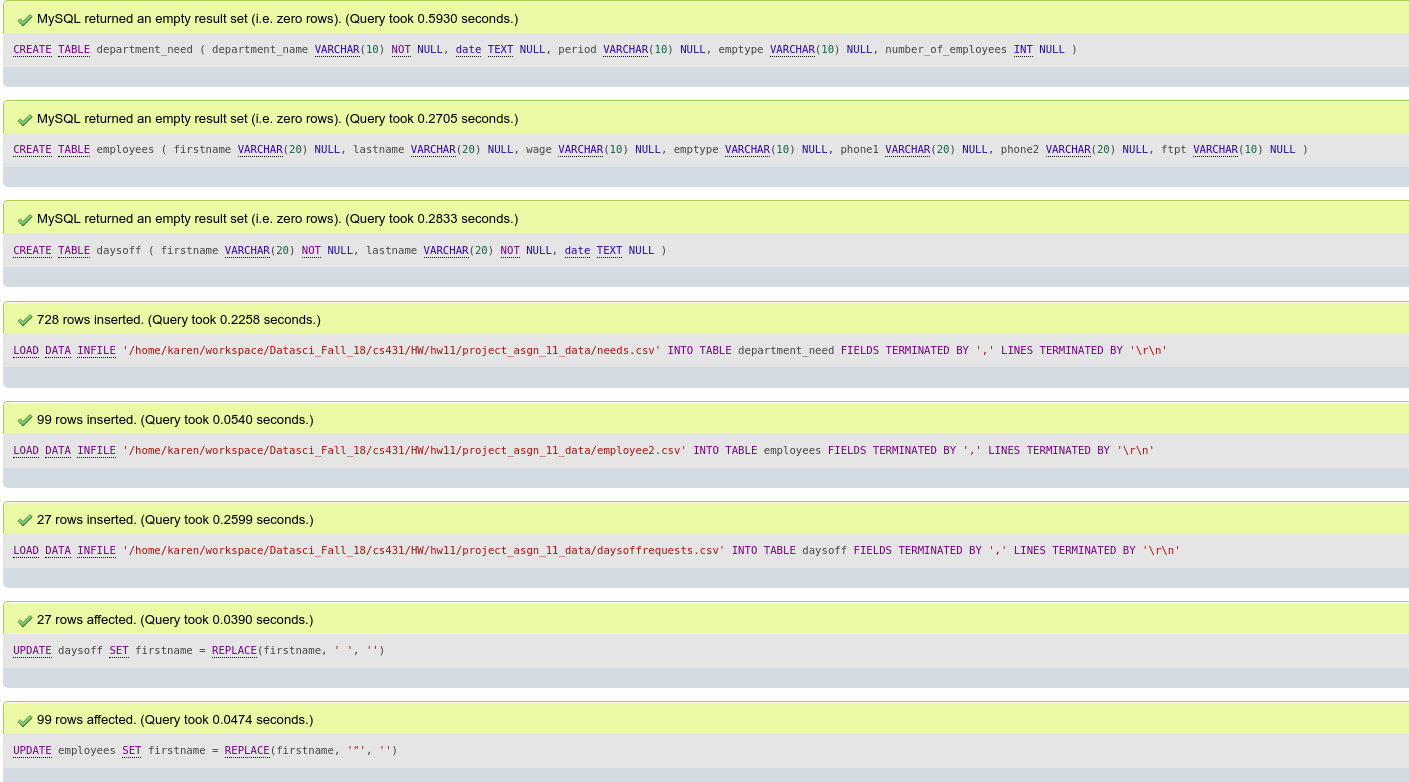
\includegraphics{2.png}
\caption{}
\end{figure}

\begin{figure}[H]
\centering
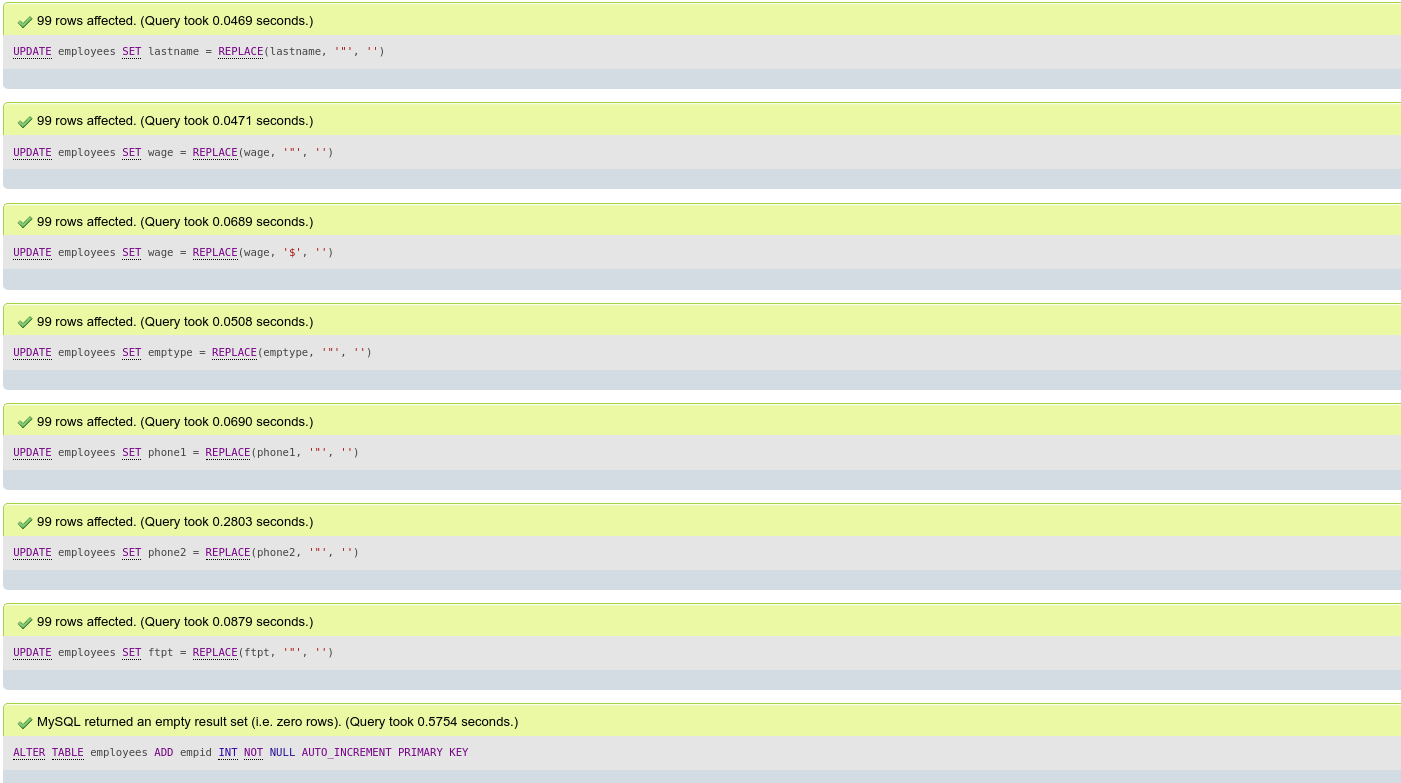
\includegraphics{3.png}
\caption{}
\end{figure}

\begin{figure}[H]
\centering
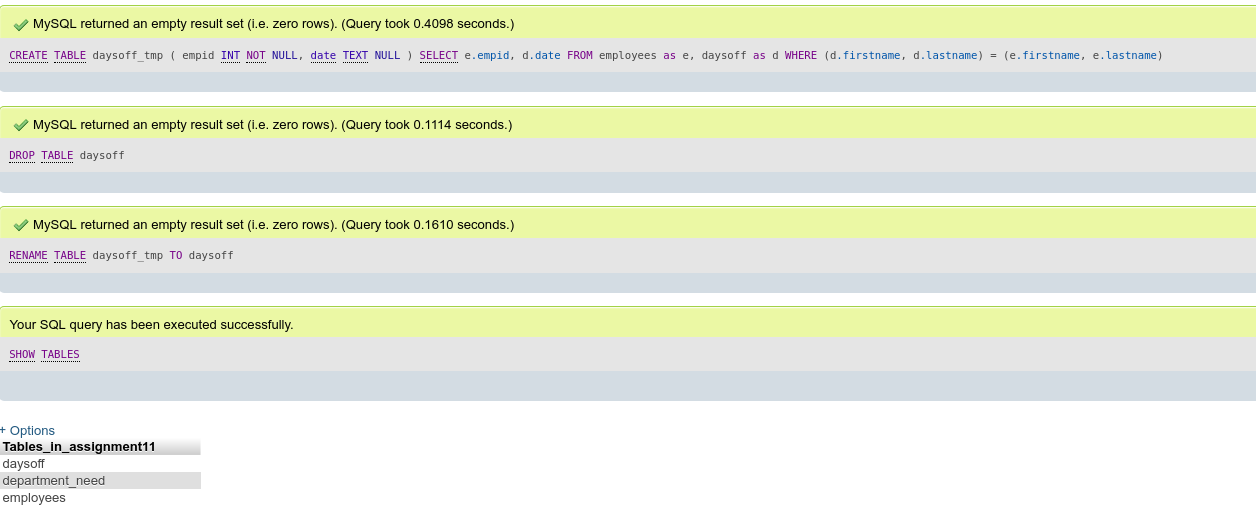
\includegraphics{4.png}
\caption{}
\end{figure}

\begin{figure}[H]
\centering
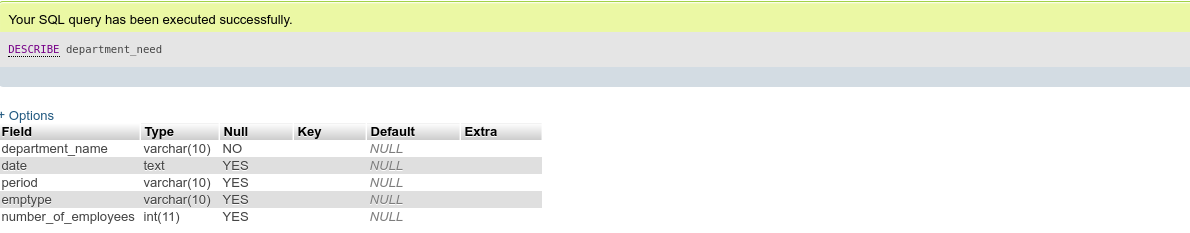
\includegraphics{5.png}
\caption{}
\end{figure}

\begin{figure}[H]
\centering
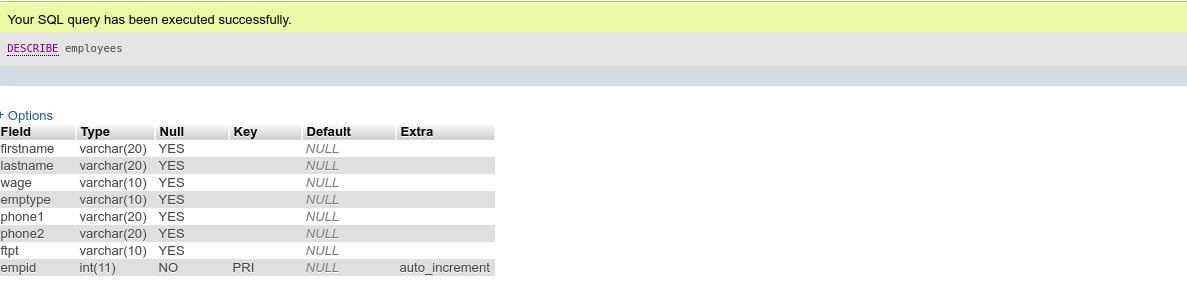
\includegraphics{6.png}
\caption{}
\end{figure}

\begin{figure}[H]
\centering
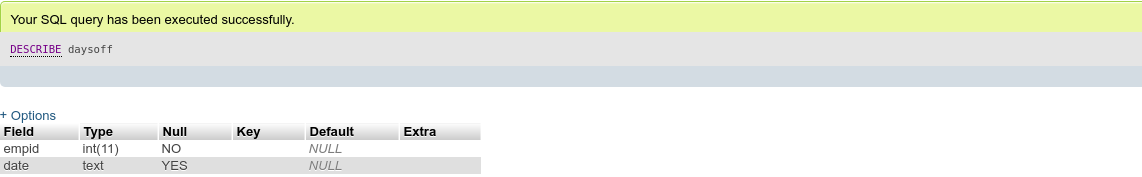
\includegraphics{7.png}
\caption{}
\end{figure}

    \subsection*{Q3}\label{q3}

Calculate the total needs of all departments, all days, all shifts by
employee type. For example: RNs: 3214 hours, LPNs: 2735 hours, etc.

    \begin{Verbatim}[commandchars=\\\{\}]
{\color{incolor}In [{\color{incolor} }]:} \PY{n}{SELECT} \PY{n}{emptype}\PY{p}{,} \PY{n}{cast}\PY{p}{(}\PY{n}{SUM}\PY{p}{(}\PY{n}{shifthrs}\PY{p}{)} \PY{n}{AS} \PY{n}{INT}\PY{p}{)} \PY{n}{AS} \PY{n}{total\PYZus{}working\PYZus{}hrs}
        \PY{n}{FROM}
          \PY{p}{(}\PY{n}{SELECT} \PY{n}{emptype}\PY{p}{,}
            \PY{l+m+mi}{8}\PY{o}{*}\PY{n}{number\PYZus{}of\PYZus{}employees} \PY{n}{AS} \PY{n}{shifthrs}
           \PY{n}{FROM} \PY{n}{department\PYZus{}need}\PY{p}{)} \PY{k}{as} \PY{n}{tmp}
        \PY{n}{GROUP} \PY{n}{BY} \PY{n}{emptype}\PY{p}{;}
\end{Verbatim}

    \begin{figure}[H]
\centering
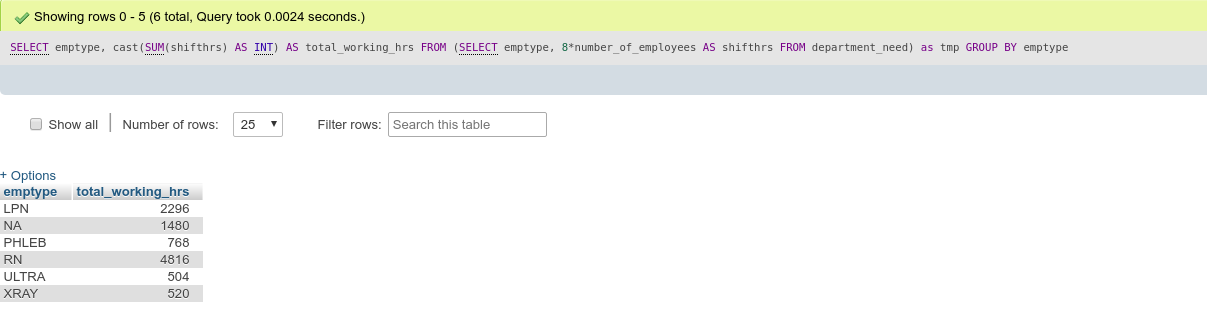
\includegraphics{8.png}
\caption{}
\end{figure}



    \subsection*{Q4}\label{q4}

Calculate the total available hours per employee type. For example: RNs:
3000 hours, LPNs: 2800 hours. Note that a part-time person is limited to
24 hours per week. Also note that requested time off is not figured into
this calculation.

    \begin{Verbatim}[commandchars=\\\{\}]
{\color{incolor}In [{\color{incolor} }]:} \PY{n}{SELECT} \PY{n}{emptype}\PY{p}{,} \PY{n}{cast}\PY{p}{(}\PY{n+nb}{sum}\PY{p}{(}\PY{n}{each\PYZus{}hrs}\PY{p}{)} \PY{n}{AS} \PY{n}{INT}\PY{p}{)} \PY{k}{as} \PY{n}{total\PYZus{}available\PYZus{}hrs}
        \PY{n}{FROM} \PY{p}{(}\PY{n}{SELECT} \PY{n}{empid}\PY{p}{,} \PY{n}{emptype}\PY{p}{,} \PY{n}{ftpt}\PY{p}{,} \PY{k}{if}\PY{p}{(}\PY{n}{ftpt}\PY{o}{=}\PY{l+s+s1}{\PYZsq{}}\PY{l+s+s1}{FT}\PY{l+s+s1}{\PYZsq{}}\PY{p}{,} \PY{n}{available\PYZus{}days}\PY{o}{*}\PY{l+m+mi}{8}\PY{p}{,} \PY{n}{available\PYZus{}days}\PY{o}{*}\PY{l+m+mf}{(24/7)}\PY{p}{)}
        \PY{k}{as} \PY{n}{each\PYZus{}hrs}
               \PY{n}{FROM} \PY{p}{(}\PY{n}{SELECT} \PY{n}{e}\PY{o}{.}\PY{n}{empid}\PY{p}{,} \PY{n}{e}\PY{o}{.}\PY{n}{emptype}\PY{p}{,} \PY{n}{e}\PY{o}{.}\PY{n}{ftpt}\PY{p}{,}
                     \PY{k}{if}\PY{p}{(}\PY{n}{isnull}\PY{p}{(}\PY{n}{agg\PYZus{}daysoff}\PY{o}{.}\PY{n}{dayoff}\PY{p}{)}\PY{p}{,} \PY{l+m+mi}{0}\PY{p}{,} \PY{n}{agg\PYZus{}daysoff}\PY{o}{.}\PY{n}{dayoff}\PY{p}{)} \PY{k}{as} \PY{n}{requested\PYZus{}day\PYZus{}off}\PY{p}{,}
                     \PY{k}{if}\PY{p}{(}\PY{n}{isnull}\PY{p}{(}\PY{n}{agg\PYZus{}daysoff}\PY{o}{.}\PY{n}{dayoff}\PY{p}{)}\PY{p}{,} \PY{l+m+mi}{14}\PY{p}{,} \PY{l+m+mi}{14} \PY{o}{\PYZhy{}} \PY{n}{agg\PYZus{}daysoff}\PY{o}{.}\PY{n}{dayoff}\PY{p}{)} \PY{k}{as} \PY{n}{available\PYZus{}days}
                     \PY{n}{FROM} \PY{n}{employees} \PY{k}{as} \PY{n}{e}
                     \PY{n}{LEFT} \PY{n}{JOIN} \PY{p}{(}\PY{n}{SELECT} \PY{n}{empid}\PY{p}{,} \PY{n}{count}\PY{p}{(}\PY{o}{*}\PY{p}{)} \PY{k}{as} \PY{n}{dayoff}
                                \PY{n}{FROM} \PY{n}{daysoff}
                                \PY{n}{GROUP} \PY{n}{BY} \PY{n}{empid}\PY{p}{)} \PY{k}{as} \PY{n}{agg\PYZus{}daysoff}
                     \PY{n}{ON} \PY{n}{e}\PY{o}{.}\PY{n}{empid}\PY{o}{=}\PY{n}{agg\PYZus{}daysoff}\PY{o}{.}\PY{n}{empid}\PY{p}{)} \PY{k}{as} \PY{n}{tmp1}\PY{p}{)} \PY{k}{as} \PY{n}{tmp2}
        \PY{n}{GROUP} \PY{n}{BY} \PY{n}{emptype}\PY{p}{;}
\end{Verbatim}

    \begin{figure}[H]
\centering
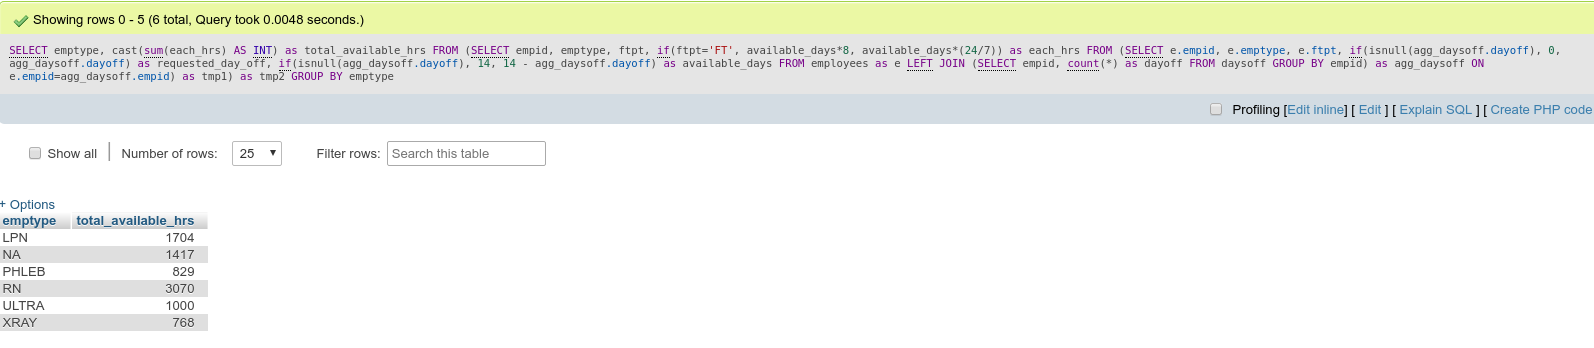
\includegraphics{9.png}
\caption{}
\end{figure}


    \subsection*{Q5}\label{q5}

List (via PHP/SQL code) which employee types are short-staffed (you
don't have enough possible hours to fill the needs for that employee
type).

    \begin{Verbatim}[commandchars=\\\{\}]
{\color{incolor}In [{\color{incolor} }]:} \PY{n}{SELECT} \PY{n}{table1}\PY{o}{.}\PY{n}{emptype}\PY{p}{,}
               \PY{n}{table1}\PY{o}{.}\PY{n}{total\PYZus{}working\PYZus{}hrs}\PY{p}{,}
               \PY{n}{table2}\PY{o}{.}\PY{n}{total\PYZus{}available\PYZus{}hrs}\PY{p}{,}
               \PY{k}{if}\PY{p}{(}\PY{n}{table2}\PY{o}{.}\PY{n}{total\PYZus{}available\PYZus{}hrs}\PY{o}{\PYZlt{}}\PY{n}{table1}\PY{o}{.}\PY{n}{total\PYZus{}working\PYZus{}hrs}\PY{p}{,} \PY{l+s+s1}{\PYZsq{}}\PY{l+s+s1}{YES}\PY{l+s+s1}{\PYZsq{}}\PY{p}{,} \PY{l+s+s1}{\PYZsq{}}\PY{l+s+s1}{NO}\PY{l+s+s1}{\PYZsq{}}\PY{p}{)} \PY{k}{as} \PY{n}{short\PYZus{}staffed}
        \PY{n}{FROM} \PY{p}{(}\PY{n}{SELECT} \PY{n}{emptype}\PY{p}{,} \PY{n}{cast}\PY{p}{(}\PY{n}{SUM}\PY{p}{(}\PY{n}{shifthrs}\PY{p}{)} \PY{n}{AS} \PY{n}{INT}\PY{p}{)} 
        \PY{n}{AS} \PY{n}{total\PYZus{}working\PYZus{}hrs}
              \PY{n}{FROM}
                \PY{p}{(}\PY{n}{SELECT} \PY{n}{emptype}\PY{p}{,}
                   \PY{l+m+mi}{8}\PY{o}{*}\PY{n}{number\PYZus{}of\PYZus{}employees} \PY{n}{AS} \PY{n}{shifthrs}
                 \PY{n}{FROM} \PY{n}{department\PYZus{}need}\PY{p}{)} \PY{k}{as} \PY{n}{tmp}
              \PY{n}{GROUP} \PY{n}{BY} \PY{n}{emptype}\PY{p}{)} \PY{k}{as} \PY{n}{table1}
        \PY{n}{INNER} \PY{n}{JOIN}
          \PY{p}{(}\PY{n}{SELECT} \PY{n}{emptype}\PY{p}{,} \PY{n}{cast}\PY{p}{(}\PY{n+nb}{sum}\PY{p}{(}\PY{n}{each\PYZus{}hrs}\PY{p}{)} \PY{n}{AS} \PY{n}{INT}\PY{p}{)} 
          \PY{k}{as} \PY{n}{total\PYZus{}available\PYZus{}hrs}
           \PY{n}{FROM} \PY{p}{(}\PY{n}{SELECT} \PY{n}{empid}\PY{p}{,} \PY{n}{emptype}\PY{p}{,} \PY{n}{ftpt}\PY{p}{,} \PY{k}{if}\PY{p}{(}\PY{n}{ftpt}\PY{o}{=}\PY{l+s+s1}{\PYZsq{}}\PY{l+s+s1}{FT}\PY{l+s+s1}{\PYZsq{}}\PY{p}{,} \PY{n}{available\PYZus{}days}\PY{o}{*}\PY{l+m+mi}{8}\PY{p}{,} \PY{n}{available\PYZus{}days}\PY{o}{*}\PY{l+m+mf}{(24/7)}\PY{p}{)}
           		 \PY{k}{as} \PY{n}{each\PYZus{}hrs}
                 \PY{n}{FROM} \PY{p}{(}\PY{n}{SELECT} \PY{n}{e}\PY{o}{.}\PY{n}{empid}\PY{p}{,} \PY{n}{e}\PY{o}{.}\PY{n}{emptype}\PY{p}{,} \PY{n}{e}\PY{o}{.}\PY{n}{ftpt}\PY{p}{,}
                         \PY{k}{if}\PY{p}{(}\PY{n}{isnull}\PY{p}{(}\PY{n}{agg\PYZus{}daysoff}\PY{o}{.}\PY{n}{dayoff}\PY{p}{)}\PY{p}{,} \PY{l+m+mi}{0}\PY{p}{,} \PY{n}{agg\PYZus{}daysoff}\PY{o}{.}\PY{n}{dayoff}\PY{p}{)} \PY{k}{as} \PY{n}{requested\PYZus{}day\PYZus{}off}\PY{p}{,}
                         \PY{k}{if}\PY{p}{(}\PY{n}{isnull}\PY{p}{(}\PY{n}{agg\PYZus{}daysoff}\PY{o}{.}\PY{n}{dayoff}\PY{p}{)}\PY{p}{,} \PY{l+m+mi}{14}\PY{p}{,} \PY{l+m+mi}{14} \PY{o}{\PYZhy{}} \PY{n}{agg\PYZus{}daysoff}\PY{o}{.}\PY{n}{dayoff}\PY{p}{)} \PY{k}{as} \PY{n}{available\PYZus{}days}
                       \PY{n}{FROM} \PY{n}{employees} \PY{k}{as} \PY{n}{e}
                         \PY{n}{LEFT} \PY{n}{JOIN} \PY{p}{(}\PY{n}{SELECT} \PY{n}{empid}\PY{p}{,} \PY{n}{count}\PY{p}{(}\PY{o}{*}\PY{p}{)} \PY{k}{as} \PY{n}{dayoff}
                                    \PY{n}{FROM} \PY{n}{daysoff}
                                    \PY{n}{GROUP} \PY{n}{BY} \PY{n}{empid}\PY{p}{)} \PY{k}{as} \PY{n}{agg\PYZus{}daysoff}
                           \PY{n}{ON} \PY{n}{e}\PY{o}{.}\PY{n}{empid}\PY{o}{=}\PY{n}{agg\PYZus{}daysoff}\PY{o}{.}\PY{n}{empid}\PY{p}{)} \PY{k}{as} \PY{n}{tmp1}\PY{p}{)} \PY{k}{as} \PY{n}{tmp2}
           \PY{n}{GROUP} \PY{n}{BY} \PY{n}{emptype}\PY{p}{)} \PY{k}{as} \PY{n}{table2}
        \PY{n}{ON} \PY{n}{table1}\PY{o}{.}\PY{n}{emptype}\PY{o}{=}\PY{n}{table2}\PY{o}{.}\PY{n}{emptype}\PY{p}{;}
\end{Verbatim}

    \begin{figure}[H]
\centering
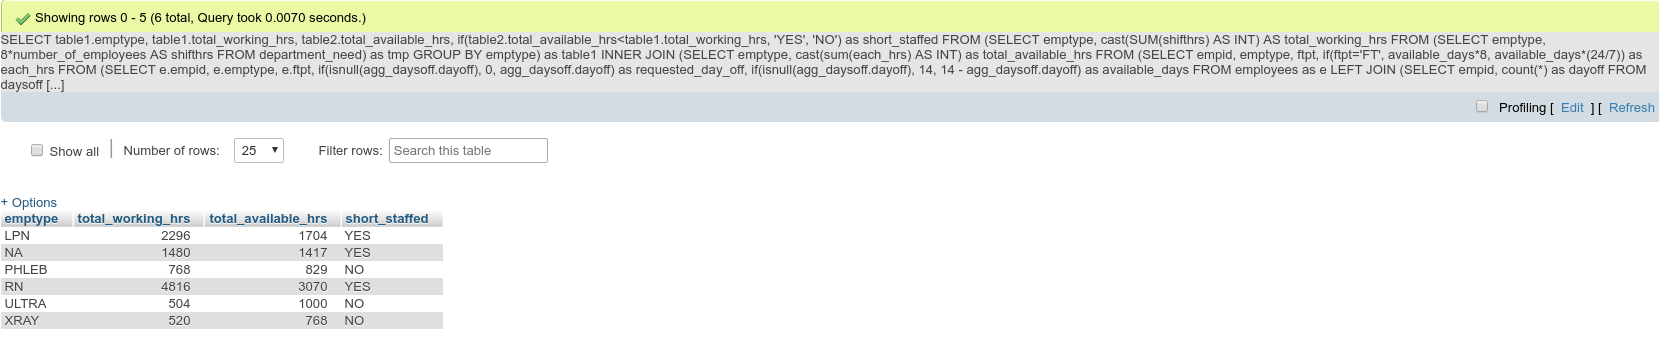
\includegraphics{10.png}
\caption{}
\end{figure}

    \subsection*{Q6}\label{q6}

Calculate the average cost per hour for each employee type, then use
that number to estimate the total cost for each employee type for the
entire schedule.

    \begin{Verbatim}[commandchars=\\\{\}]
{\color{incolor}In [{\color{incolor} }]:} \PY{n}{SELECT} \PY{n}{table1}\PY{o}{.}\PY{n}{emptype}\PY{p}{,}
               \PY{n}{table2}\PY{o}{.}\PY{n}{total\PYZus{}working\PYZus{}hrs}\PY{p}{,}
               \PY{n}{concat}\PY{p}{(}\PY{l+s+s1}{\PYZsq{}}\PY{l+s+s1}{\PYZdl{}}\PY{l+s+s1}{\PYZsq{}}\PY{p}{,} \PY{n}{table1}\PY{o}{.}\PY{n}{avg\PYZus{}wage}\PY{p}{)} \PY{k}{as} \PY{n}{avg\PYZus{}wage}\PY{p}{,}
               \PY{n}{concat}\PY{p}{(}\PY{l+s+s1}{\PYZsq{}}\PY{l+s+s1}{\PYZdl{}}\PY{l+s+s1}{\PYZsq{}}\PY{p}{,} \PY{n}{table2}\PY{o}{.}\PY{n}{total\PYZus{}working\PYZus{}hrs}\PY{o}{*}\PY{n}{table1}\PY{o}{.}\PY{n}{avg\PYZus{}wage}\PY{p}{)} \PY{k}{as} \PY{n}{total\PYZus{}cost}
        \PY{n}{FROM} \PY{p}{(}\PY{n}{SELECT} \PY{n}{emptype}\PY{p}{,} \PY{n+nb}{round}\PY{p}{(}\PY{n}{avg}\PY{p}{(}\PY{n}{wage}\PY{p}{)}\PY{p}{,} \PY{l+m+mi}{3}\PY{p}{)} \PY{k}{as} \PY{n}{avg\PYZus{}wage}
              \PY{n}{FROM} \PY{n}{employees}
              \PY{n}{GROUP} \PY{n}{BY} \PY{n}{emptype}\PY{p}{)} \PY{k}{as} \PY{n}{table1}
        \PY{n}{INNER} \PY{n}{JOIN}
          \PY{p}{(}\PY{n}{SELECT} \PY{n}{emptype}\PY{p}{,} \PY{n}{cast}\PY{p}{(}\PY{n}{SUM}\PY{p}{(}\PY{n}{shifthrs}\PY{p}{)} \PY{n}{AS} \PY{n}{INT}\PY{p}{)} \PY{n}{AS} \PY{n}{total\PYZus{}working\PYZus{}hrs}
                    \PY{n}{FROM}
                      \PY{p}{(}\PY{n}{SELECT} \PY{n}{emptype}\PY{p}{,}
                         \PY{l+m+mi}{8}\PY{o}{*}\PY{n}{number\PYZus{}of\PYZus{}employees} \PY{n}{AS} \PY{n}{shifthrs}
                       \PY{n}{FROM} \PY{n}{department\PYZus{}need}\PY{p}{)} \PY{k}{as} \PY{n}{tmp}
                    \PY{n}{GROUP} \PY{n}{BY} \PY{n}{emptype}\PY{p}{)} \PY{k}{as} \PY{n}{table2}
        \PY{n}{ON} \PY{n}{table1}\PY{o}{.}\PY{n}{emptype} \PY{o}{=} \PY{n}{table2}\PY{o}{.}\PY{n}{emptype}\PY{p}{;}
\end{Verbatim}

    \begin{figure}[H]
\centering
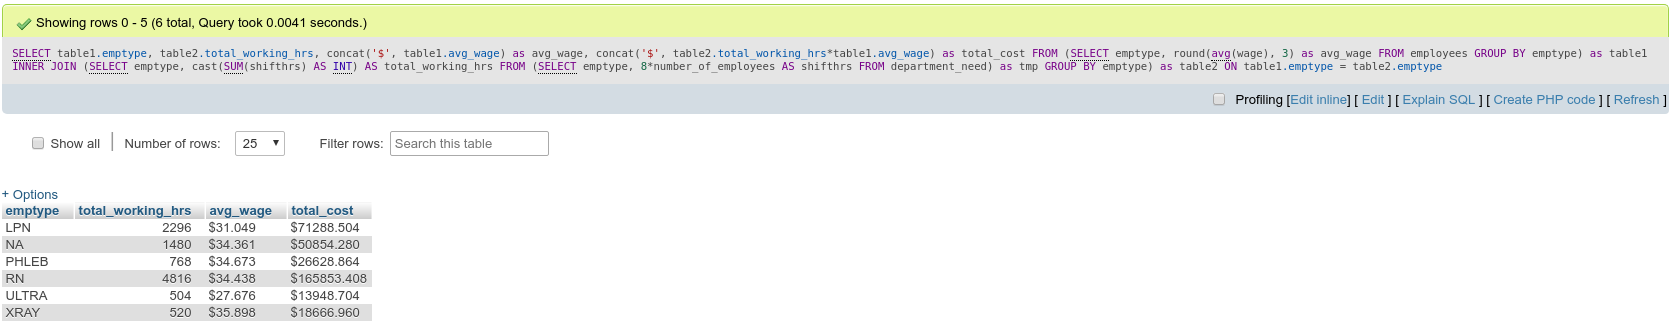
\includegraphics{11.png}
\caption{}
\end{figure}

    \subsection*{Q7}\label{q7}

For all full time employees, calculate the total cost of giving them the
day off. This assumes that they get paid time off, and that they will be
paid for one, 8-hour shift.

    \begin{Verbatim}[commandchars=\\\{\}]
{\color{incolor}In [{\color{incolor} }]:} \PY{n}{SELECT} \PY{n}{table1}\PY{o}{.}\PY{n}{empid}\PY{p}{,}
               \PY{n}{table1}\PY{o}{.}\PY{n}{wage} \PY{k}{as} \PY{n}{wage\PYZus{}per\PYZus{}hour}\PY{p}{,}
               \PY{n}{table2}\PY{o}{.}\PY{n}{dayoff} \PY{k}{as} \PY{n}{number\PYZus{}of\PYZus{}daysoff}\PY{p}{,}
               \PY{n+nb}{round}\PY{p}{(}\PY{n}{table2}\PY{o}{.}\PY{n}{dayoff}\PY{o}{*}\PY{n}{table1}\PY{o}{.}\PY{n}{wage}\PY{o}{*}\PY{l+m+mi}{8}\PY{p}{,}\PY{l+m+mi}{3}\PY{p}{)} \PY{k}{as} \PY{n}{cost\PYZus{}of\PYZus{}paid\PYZus{}dayoff}
        \PY{n}{FROM}
          \PY{p}{(}\PY{n}{SELECT} \PY{n}{empid}\PY{p}{,} \PY{n}{wage}
           \PY{n}{FROM} \PY{n}{employees}
           \PY{n}{WHERE} \PY{n}{ftpt}\PY{o}{=}\PY{l+s+s1}{\PYZsq{}}\PY{l+s+s1}{FT}\PY{l+s+s1}{\PYZsq{}}\PY{p}{)} \PY{k}{as} \PY{n}{table1}
        \PY{n}{INNER} \PY{n}{JOIN}
          \PY{p}{(}\PY{n}{SELECT} \PY{n}{empid}\PY{p}{,} \PY{n}{count}\PY{p}{(}\PY{o}{*}\PY{p}{)} \PY{k}{as} \PY{n}{dayoff}
           \PY{n}{FROM} \PY{n}{daysoff}
           \PY{n}{GROUP} \PY{n}{BY} \PY{n}{empid}\PY{p}{)} \PY{k}{as} \PY{n}{table2}
        \PY{n}{ON} \PY{n}{table1}\PY{o}{.}\PY{n}{empid}\PY{o}{=}\PY{n}{table2}\PY{o}{.}\PY{n}{empid}\PY{p}{;}
\end{Verbatim}

    \begin{figure}[H]
\centering
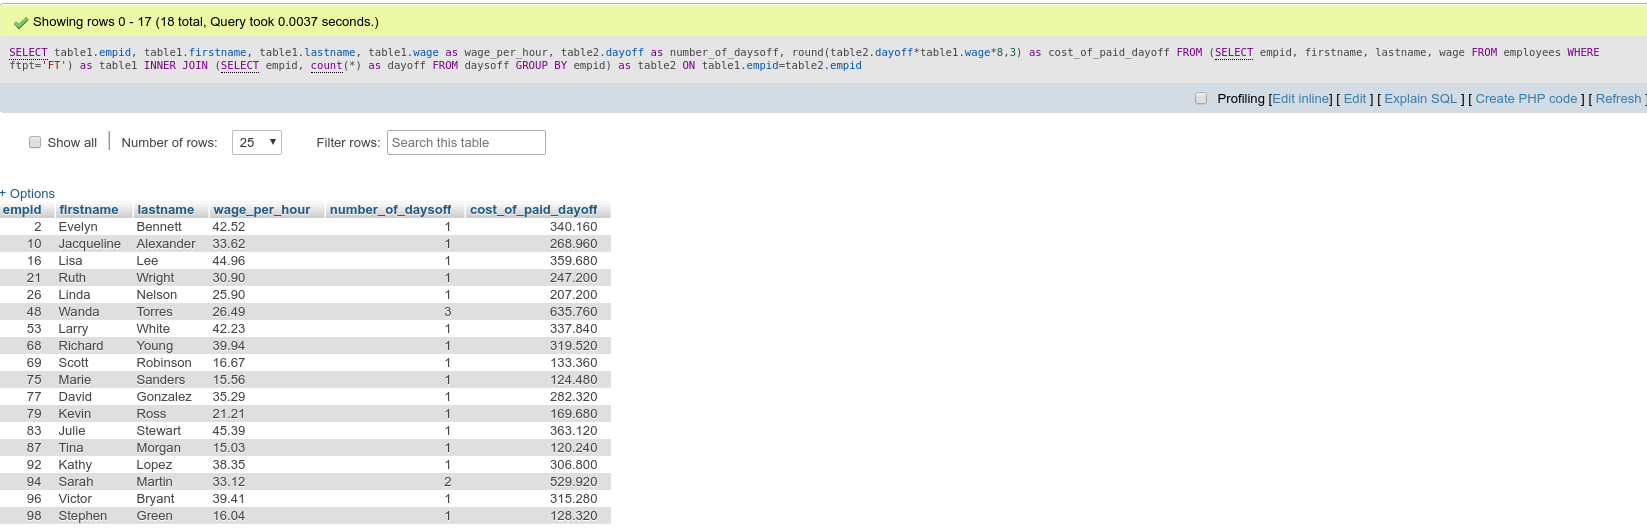
\includegraphics{12.png}
\caption{}
\end{figure}


    % Add a bibliography block to the postdoc
    
    
    
    \end{document}
